\chapter{ANEXOS}
\section{Rendimiento formato de comprensi\'on Tariy - Formato ARFF}

Un an\'alisis del formato para compresi\'on de datos descrito en el Cap\'itulo 7 del presente trabajo, en la
secci\'on Arquitectura Tariy, con respecto al formato ARFF de la herramienta de Miner\'ia de Datos WEKA se
muestra en el siguiente cuadro, donde se registra el tama\~no en disco de cada formato al almacenar conjuntos de
datos con diferente n\'umero de transacciones y atributos.

\begin{table}[h]
\caption{An\'alisis formatos de almacenamiento}
\label{formatos}
\end{table}
\begin{center}
\begin{tabular}{|p{30mm}|p{20mm}|p{20mm}|p{20mm}|p{20mm}|} \hline
\textbf{Archivo ARFF}    & \textbf{N\'um. Instancias} & \textbf{N\'um. Atributos} & \textbf{Tam. ARFF (KB)} &
\textbf{Tam. Tariy (KB)}\\ \hline
mushroom        & 8124              & 23               & 726.30         & 133.81\\ \hline
titanic         & 2201              &  4               &  64.60         &   0.17\\ \hline
tictactoe       &  958              & 10               &  26.50         &  14.00\\ \hline
soybean         &  683              & 36               & 194.10         &  55.46\\ \hline
vote            &  435              & 17               &  32.20         &   8.87\\ \hline
contact-lenses  &   24              &  5               &   1.10         &   0.23\\ \hline
weather.nominal &   14              &  5               &   0.57         &   0.16\\ \hline
\end{tabular}
\end{center}

\begin{figure}[h]
\centering
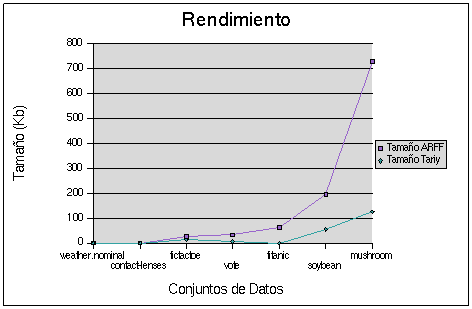
\includegraphics[width=0.7\textwidth]{images/formatos.png}
\caption{Rendimiento formatos de almacenamiento}
\end{figure}
